Dans ce chapitre nous allons faire le tour des différentes décisions techniques
prises, et outils utilisés.

Nous allons commencer par présenter les technologies utilisées, puis nous allons parler du choix
architectural de l'application, et enfin nous allons parler des différents modèles utilisés.

\section{Choix techniques et motivations}\label{sec: conception-choix-techniques-et-motivation}
\subsection{MySQL}\label{subsec:conception-mysql}
Le choix de la base de données est une étape importante dans le développement
d'une application.

Il existe plusieurs types de bases de données, chacune avec
ses propres avantages et inconvénients.

Dans ce projet, nous avons choisi
d'utiliser une base de données relationnelle, car elle est la plus adaptée à
notre cas d'utilisation.

Elle nous permet de stocker les données de manière
structurée, et de les manipuler facilement à l'aide de requêtes SQL. Nous avons
choisi d'utiliser MysQL, car c'est une base de données relationnelle
populaire, avec une grande communauté de développeurs
et une documentation complète.


\subsection{Architecture de l'application}\label{subsec: conception-application-architecture}
Nous avons choisi une architecture client-serveur pour notre application. Le
serveur est responsable de la logique métier et de la gestion des données, et
le client est responsable de l'interface utilisateur. Le client communique avec
le serveur via une API REST (Representational State Transfer), qui est un
ensemble de conventions et de bonnes pratiques pour la conception d'API web.
L'API REST permet au client d'effectuer des opérations CRUD (Create, Read,
Update, Delete) sur les données stockées sur le serveur. Nous avons choisi
d'utiliser une API REST, car elle est simple à mettre en œuvre et facile à
utiliser. Elle permet également de séparer la logique métier de l'interface
utilisateur, ce qui facilite la maintenance et l'évolutivité de l'application.
Nous avons choisi d'utiliser JSON (JavaScript Object Notation) comme format de
données pour l'API REST, car il est léger, facile à lire et à écrire.

\subsection{Le processus unifié}\label{subsec: conception-unified-process}
Nous avons choisi d'utiliser le processus unifié pour le développement de
notre application. Le processus unifié est un processus de développement de
logiciels itératif et incrémental de la famille des méthodes agiles.

le processus unifié utilise des modèles UML (Unified Modeling Language) pour la
conception et la modélisation.

\subsection{Typescript}\label{subsec: conception-typescript}
Nous avons choisi d'utiliser Typescript pour le développement de notre
application. Typescript est un langage de programmation open source développé
par Microsoft. Il est conçu pour le développement d'applications JavaScript
à grande échelle. Il ajoute des fonctionnalités au JavaScript, comme le typage
statique, les classes, les interfaces, les modules, etc. Il est compilé en
JavaScript, et peut donc être utilisé sur n'importe quel navigateur web ou
serveur web.

Le plus gros avantages de Typescript est qu'il est facile à apprendre et à
utiliser, et il nous permet de détecter les erreurs de programmation avant
l'exécution du code, de plus il est compilé en JavaScript, et peut donc être
utilisé sur n'importe quel navigateur web ou serveur web ce qui nous permet d'avoir un
code client et serveur en Typescript on ne change donc pas de language entre le
client et le serveur.

\subsection{NestJS}\label{subsec: conception-nestjs}
Nous avons choisi d'utiliser NestJS pour le développement l'API(partie serveur).
NestJS est un framework open source pour le développement d'applications
Node.js. Il est basé sur Express, et utilise Typescript. Il est conçu pour
créer des applications évolutives et efficaces. Il utilise une architecture
modulaire, et est composé de plusieurs modules, chacun avec sa propre
fonctionnalité.

\subsection{NextJs}\label{subsec: conception-nextjs}
Nous avons choisi d'utiliser NextJS pour le développement de notre interface utilisateur (partie client).
web. NextJS est un framework open source pour le développement d'applications
React. Il est basé sur React, et utilise Typescript.

\subsection{Git}\label{subsec: conception-git}
Nous avons choisi d'utiliser Git pour la gestion de version de notre code. Git
est un système de contrôle de version distribué open source. Il est conçu pour
gérer les petits et grands projets avec rapidité et efficacité. Il est
utilisé pour suivre les modifications apportées au code source, et pour
faciliter la collaboration entre les développeurs. Nous avons choisi d'utiliser
Git, car il est facile à apprendre et à utiliser, et il nous permet de suivre
les modifications apportées au code source, et de revenir à une version
antérieure du code source si nécessaire.

\subsection{GitHub}\label{subsec: conception-github}
Nous avons choisi d'utiliser GitHub pour l'hébergement de notre code. GitHub est
un service d'hébergement de code source basé sur Git. Il est conçu pour
faciliter la collaboration entre les développeurs. Il est utilisé pour
héberger des projets open source et privés.

Nous avons choisi d'utiliser car ce projet est open source et nous voulons que ceux qui
souhaitent contribuer au projet puissent le faire facilement.

\subsection{Tailwindcss}\label{subsec: conception-tailwind}
Nous avons choisi d'utiliser Tailwindcss pour le développement de notre interface utilisateur (partie client).
web. Tailwindcss est un framework css pronant l'approche utility-first.

\addcontentsline{toc}{subsection}{Conclusion}
\subsection*{Conclusion}\label{subsec: conception-conclusion-choix-techniques}
Nous retiendrons par ailleurs que toutes les décisions prises ne sont pas
forcément les meilleures, mais elles ont été prises en fonction des
contraintes et des objectifs du projet.

Nous voulons non seulement résoudre le problème de la délibération, mais
aussi fournir une solution qui soit facile à maintenir et à faire évoluer à
l'avenir et facilement adaptable à d'autres problèmes similaires surtout extensible.

Le choix d'une API offre une grande flexibilité et une grande extensibilité
car la solution peut être utilisée par d'autres applications et peut être
facilement intégrée à d'autres systèmes et peut être utilisée pour concevoir
un autre type d'application (mobile, web, desktop, etc.).

\section{Modèles}\label{sec: conception-database-models}
\subsection{Diagramme de classes}\label{subsec:conception-class-diagram}
\begin{figure}[ht]
    \centering
    \caption{Diagramme de classes}
    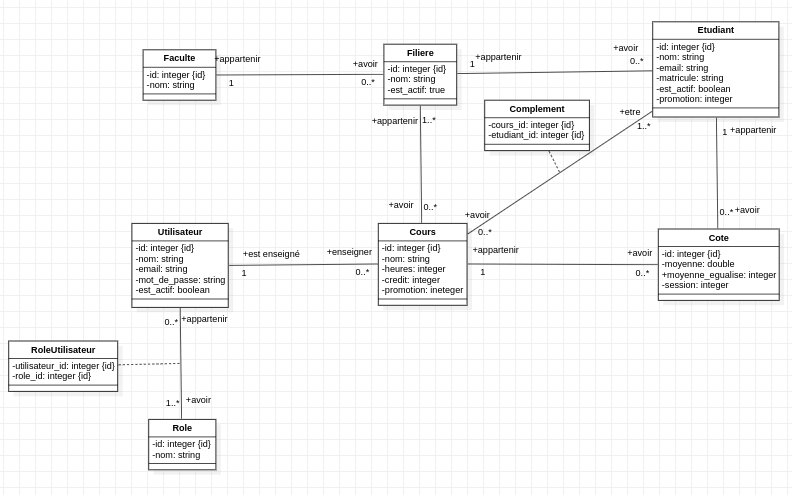
\includegraphics[width=1\linewidth]{class-diagram}
    \label{fig:class-diagram}
\end{figure}
\pagebreak

\subsection{Diagramme d'objets}\label{subsec:conception-object-diagram}
\begin{figure}[ht]
    \centering
    \caption{Diagramme d'objets}
    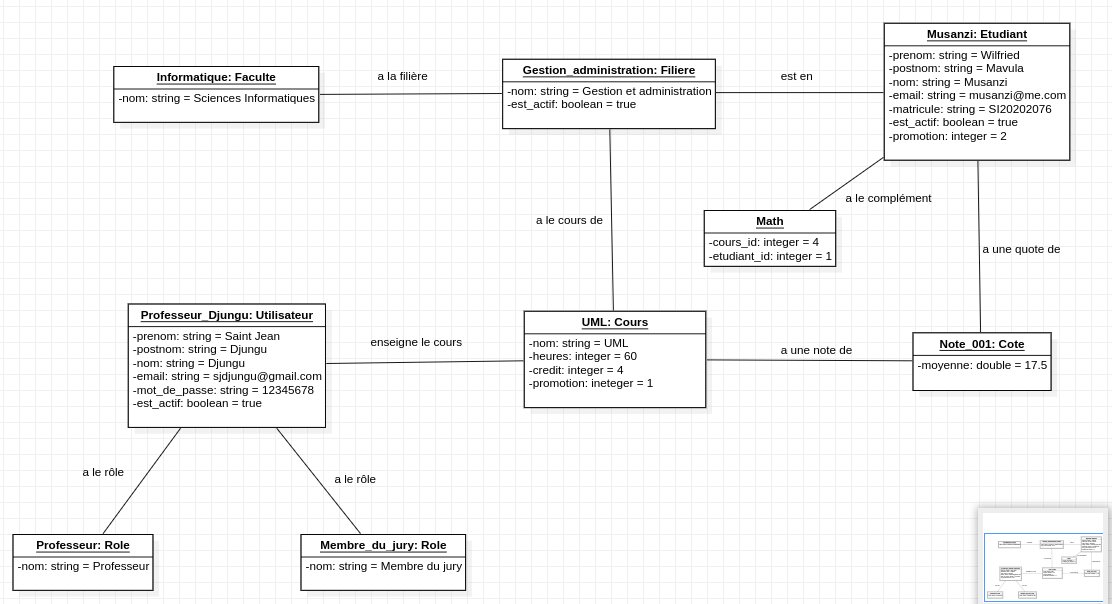
\includegraphics[width=1\linewidth]{object-diagram}
    \label{fig:object-diagram}
\end{figure}
\pagebreak


\subsection{Diagramme de cas d'utilisation}\label{subsec:conception-use-case-diagram}
\begin{figure}[ht]
    \caption{Cas d'utilisation : Gestion des facultés}
    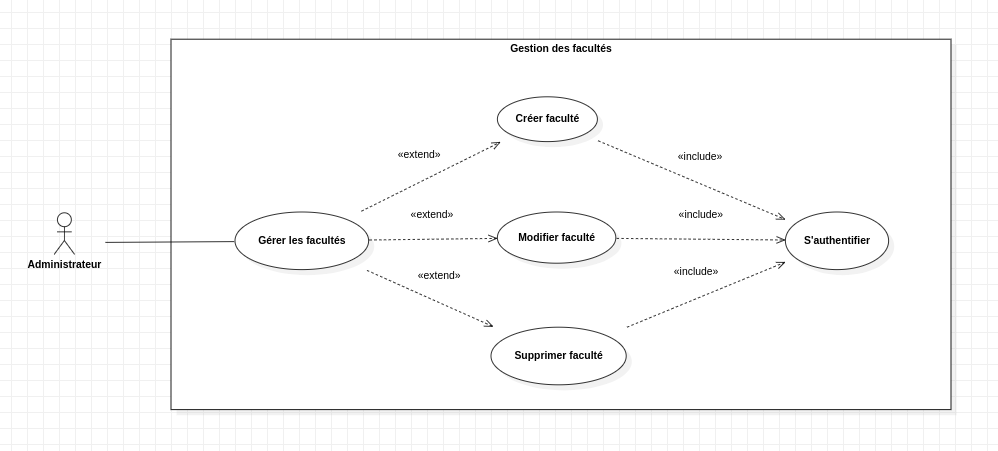
\includegraphics[width=1\linewidth]{use-cases/fac-management}
    \centering
    \label{fig:fac-management}
\end{figure}
\pagebreak

\begin{figure}[ht]
    \caption{Cas d'utilisation : Gestion des filières}
    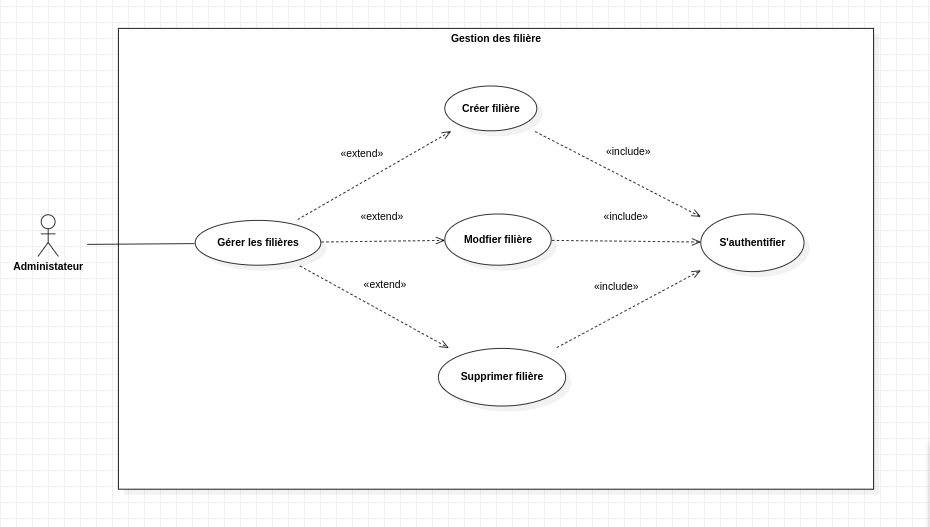
\includegraphics[width=1\linewidth]{use-cases/field-management}
    \centering
    \label{fig:field-management}
\end{figure}
\pagebreak

\begin{figure}[ht]
    \caption{Cas d'utilisation : Gestion des cours}
    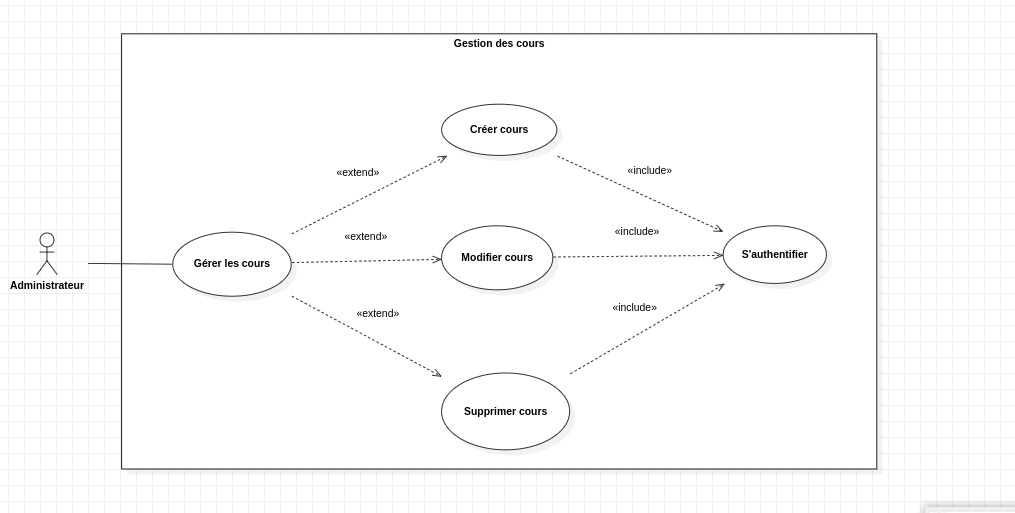
\includegraphics[width=1\linewidth]{use-cases/course-management}
    \centering
    \label{fig:course-management}
\end{figure}
\pagebreak

\begin{figure}[ht]
    \caption{Cas d'utilisation : Gestion des cotes}
    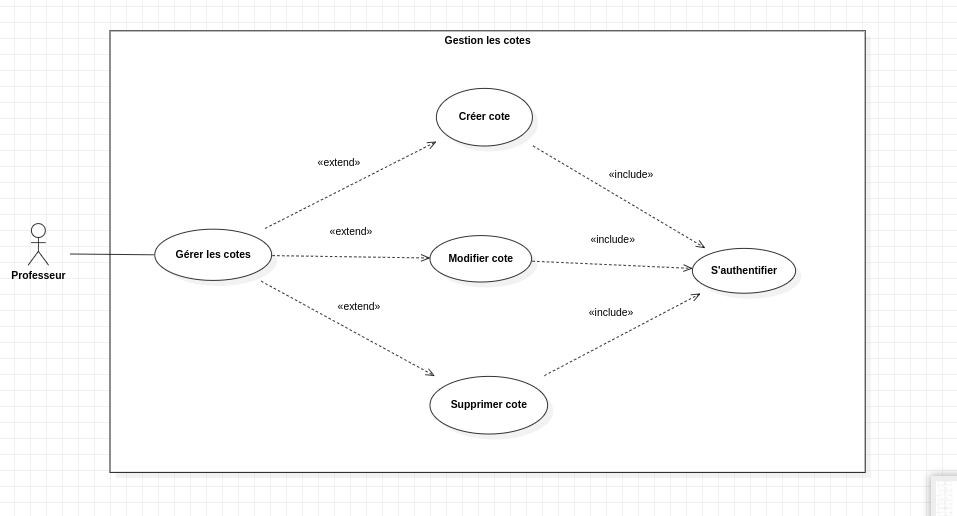
\includegraphics[width=1\linewidth]{use-cases/grades-management}
    \centering
    \label{fig:grades-management}
\end{figure}
\pagebreak

\begin{figure}[ht]
    \caption{Cas d'utilisation : Gestion des étudiants}
    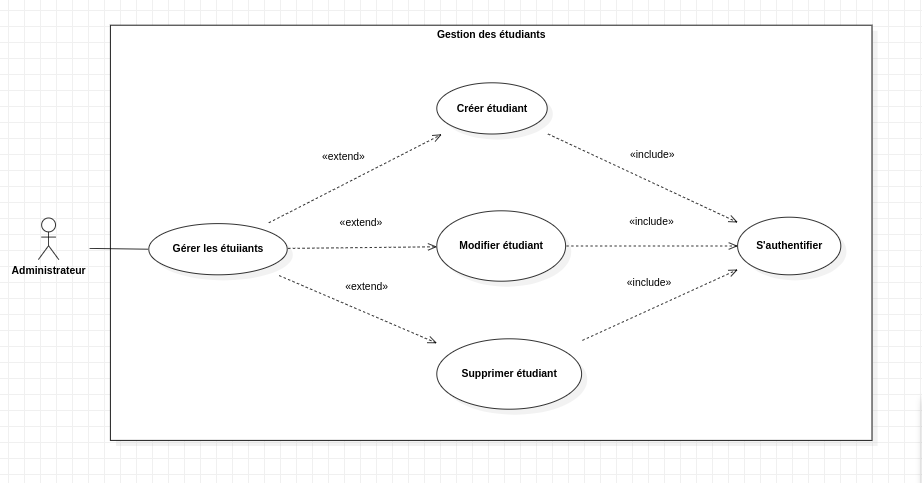
\includegraphics[width=1\linewidth]{use-cases/student-management}
    \centering
    \label{fig:student-management}
\end{figure}
\pagebreak

\begin{figure}[ht]
    \caption{Cas d'utilisation : Gestion des utilisateurs}
    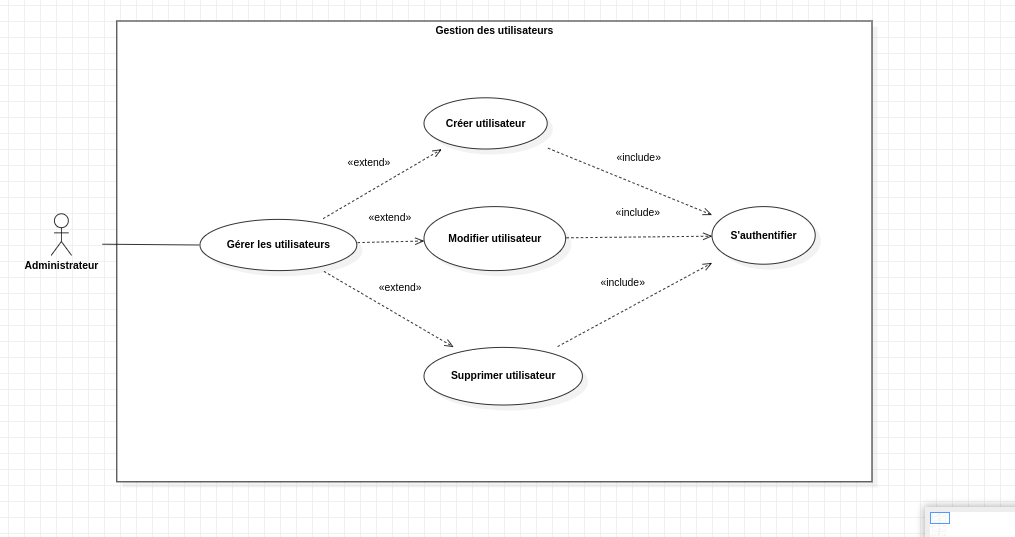
\includegraphics[width=1\linewidth]{use-cases/user-management}
    \centering
    \label{fig:user-management}
\end{figure}
\pagebreak

\begin{figure}[ht]
    \caption{Cas d'utilisation : Gestion des rôles}
    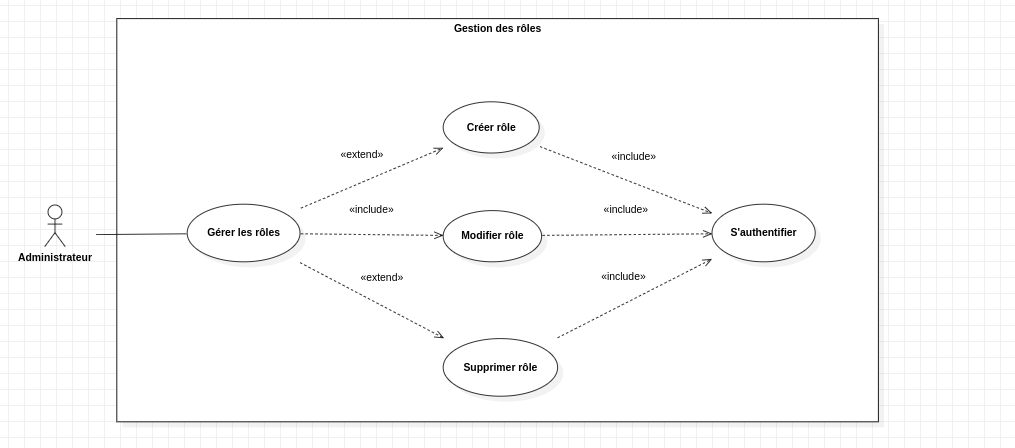
\includegraphics[width=1\linewidth]{use-cases/role-management}
    \centering
    \label{fig:role-management}
\end{figure}
\pagebreak

\begin{figure}[ht]
    \caption{Cas d'utilisation : Création des PDFs(Relevés)}
    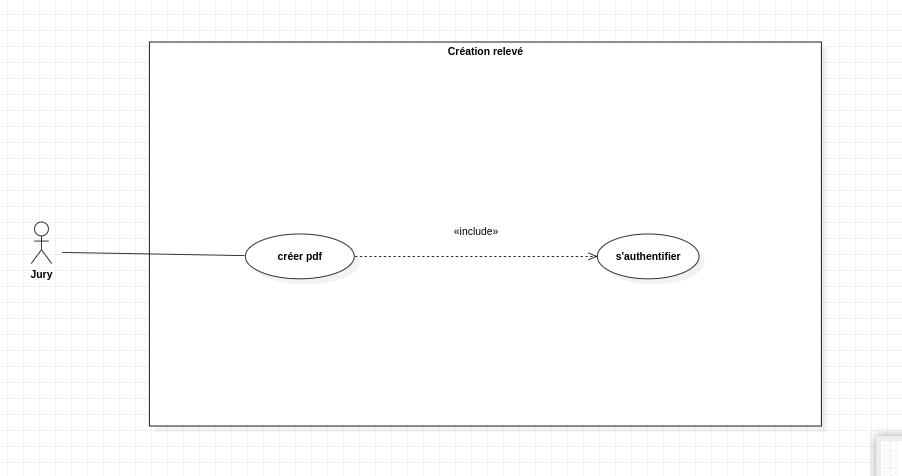
\includegraphics[width=1\linewidth]{use-cases/create-pdf}
    \centering
    \label{fig:create-pdf}
\end{figure}
\pagebreak

\begin{figure}[ht]
    \caption{Cas d'utilisation : Envoyer le pdf par mail}
    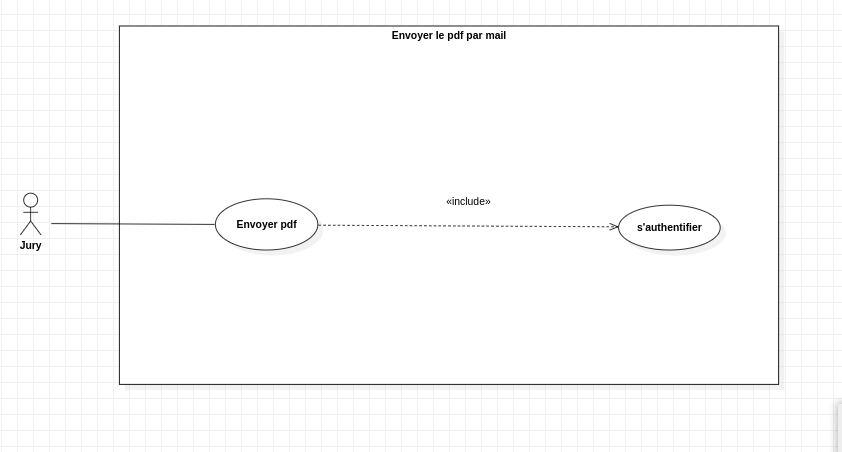
\includegraphics[width=1\linewidth]{use-cases/send-pdf}
    \centering
    \label{fig:send-pdf}
\end{figure}
\pagebreak

\subsection{Diagramme de séquence}\label{subsec:conception-sequence-diagram}
\begin{figure}[ht]
    \centering
    \caption{Diagramme de séquence}
    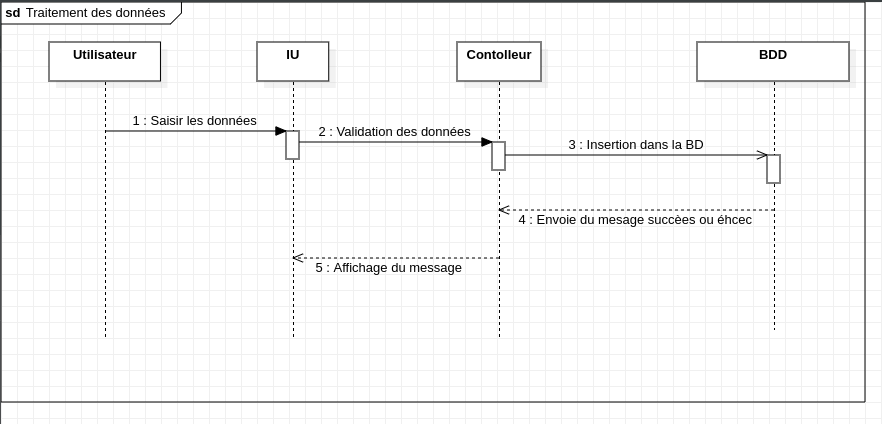
\includegraphics[width=1\linewidth]{sequence}
    \label{fig:sequence-diagram}
\end{figure}
\pagebreak